\chapter{Theory}
\label{chapter:theory}
\label{c2:theory}
In this chapter, a review is given of the theory of SEMSANS and the interpretation of measurements. First, the basic principles of SEMSANS as a neutron spin-echo technique are explained and the way the beam is modulated is derived. Next, the interaction of samples with the modulated beam is discussed, and the concept of spin-echo length $\delta$ is introduced as a way of characterizing a sample by considering its SESANS correlation function $G(\delta)$. Lastly, a reference sample used throughout this work is introduced and characterized by its $G(\delta)$ and form factor $P(Q)$. 

\section{Polarized neutrons and Larmor precession}
\label{c2.1}
Neutrons are spin $s=\frac{1}{2}$ particles with a spin angular momentum vector $\vec{S}$, the direction of $\vec{S}$ being the spin polarization $\vec{P}$. When a neutron passes through a uniform $\vec{B}$-field, $\vec{P}$ will precess by a certain angle $\phi$ over time. The frequency at which this occurs is given by
$$\omega = \gamma |B_\perp|$$
with $B_\perp$ the magnetic field strength perpendicular to the plane $\vec{P}$ is in and $\gamma$ the neutron gyromagnetic ratio. In addition to spin, a neutron has a wavelength $\lambda$ corresponding to a speed $v = \frac{h}{m\lambda}$, $m$ being the neutron mass. This means that it will pass through a uniform (perpendicular) field $B$ of length $L$ in time $t = \frac{Lm\lambda}{h}$. From this, it can be seen that the total precession will be 
\begin{equation}
	\phi = \frac{\gamma B L m\lambda}{h} = c\lambda B L \label{eq:larmor-prec}
\end{equation}
with $c = \frac{\gamma m}{h}$ being the Larmor constant \cite{bouwman2021b}.   
\section{Modulating a neutron beam using precession}
\label{c2.2}
Using the concepts of polarized neutrons and Larmor precession, the basic concept of a SEMSANS instrument can be described, deferring a detailed discussion of the source and monochromator for now. The instrument takes a neutron beamline as a source, meaning that with the choice of axes used in this research, neutrons can be assumed to move in the $z$-direction with a slight divergence in the $xy$-plane. A polarizer is used to polarize the beam in the $+x$ direction. Next, the beam passes through two precession devices  that give neutrons at wavelength $\lambda$ in the beam a $y$-dependent precession angle in the $xz$-plane due to an applied $B_y$-field %at distance $L_1, L_2$ from the detector
\begin{equation}
	\phi = 2\pi\alpha\lambda y \label{eq:precession-freq}
\end{equation}
with $\alpha$ being a constant specific to the used precession device that together with $\lambda$ determines the precession frequency. This precession can be thought of as $\vec{P}$ being rotated over a $y$-dependent angle $\phi$. Such a $y$-dependent $\phi$ is in practice created by using $B_y$-fields with interfaces at an angle $\theta_0$ with the beam axis $z$, causing $L$ in Equation \eqref{eq:larmor-prec} to vary with $y$. Different precession devices exist which can create such fields as will be analyzed and discussed in Section \ref{c3.3}.

Finally, the modulation is created by applying an analyzer to the beam afterwards \cite{mezei1972}. This again polarizes the beam in either the $+x$ or the $-x$ direction depending on the analyzer setting. Assuming a perfectly monochromatic source with wavelength $\lambda = \lambda_0$, this creates an intensity modulation pattern on the position-sensitive detector at frequency $f_0 = \alpha\lambda_0$ of the form
\begin{equation}
	I_{b,s}(y) = I_{0, b,s} \pm A_{b,s}\cos(2\pi f_0y) \label{eq:mono-modulation}
\end{equation}
where $I_{b,s}, A_{b,s}$ are experimentally observed quantities in the base case of an empty instrument ($b$) and for an instrument with a sample ($s$) and the sign of the modulation depending on the $\pm x$ analyzer setting \cite{parnell2023}. 
\section{Spin-echo length $\delta$ and measurement interpretation}
\label{c2.3}
When adding a sample to the instrument after the analyzer at distance $L_s$ from the detector, a correlation length known as the spin-echo length $\delta$ is accessed \cite{bouwman2011}, given by 
\begin{equation}
	\delta = \lambda_0^2L_s\alpha \label{eq:delta}
\end{equation}
Assuming a measurement along the $y$-axis, the above can be derived from the wave-vector transfer $Q_y$ using the small-angle expression $Q_y = \frac{2\pi}{\lambda}\frac{y}{L_s}$. In this way, $\phi$ can be rewritten to $\phi = \delta Q_y$ with $\delta$ as given. It is the same spin-echo length as used in the analysis and interpretation of SESANS \cite{rekveldt1996}\cite{krouglov2003}\cite{andersson2008}. Whereas in SESANS a decrease in overall beam polarization is used, SEMSANS considers the reduction of intensity modulation amplitude or equivalently visibility upon adding a sample, which can be shown to be related to $\delta$ through the formula \cite{parnell2023}
\begin{equation}
	\frac{A_s(\delta)}{A_b(\delta)} = P(\delta) = e^{G(\delta) - \tau} \label{eq:sample-pol-reduction}
\end{equation}
with $\tau = \sigma t$ being the scattering power, which corresponds to the average number of scattering events for a neutron traversing the sample. $t$ is the sample thickness and $\sigma$ is the total scattering cross-section defined by 
\begin{equation}
	\sigma = \frac{1}{k_0^2}\int_{-\infty}^\infty\int_{-\infty}^\infty\dfrac{d\sigma(\vec{Q})}{d\Omega}dQ_xdQ_y  \label{eq:sigma-analytical}
\end{equation}
$G(\delta)$ is the SESANS correlation function given by
\begin{equation}
	G(\delta) = \frac{t}{k_0^2}\int_{-\infty}^\infty\int_{-\infty}^\infty\dfrac{d\sigma(\vec{Q})}{d\Omega}\cos(Q_y \delta)dQ_xdQ_y  \label{eq:G-analytical}
\end{equation}
This is the 1D expression for $G(\delta)$ matching the 1D detector that will be described in the next chapter. In words, $G(\delta)$ is a cosine transform of $d\sigma(\vec{Q})/d\Omega$ \cite{li2019} along the $y$-axis with regular integration over the $x$-axis. Although formally the integration range is infinite, for practical samples the relevant $Q$-range where $d\sigma(\vec{Q})/d\Omega$ is significantly greater than zero will be limited as will be discussed for a particular sample in the next section. This makes it possible to approximate this cosine transform integral over the finite $Q$-range accessible at a detector, relying on the principle that for large enough samples most neutrons will reach the detector \cite{rekveldt1996}. This framework has been extended to 2D using a two-dimensional cosine transform, making it possible to analyze anisotropic samples using a 2D modulated beam \cite{parnell2023}.
For isotropic samples, radial integration is possible without loss of information, and $G(\delta)$ can be stated using a Hankel transform instead of a cosine transform \cite{andersson2008}.

\section{Mono-disperse reference sample and its $G(\delta)$}
\label{c2.4}
Expressions for $\tau$ and $G(\delta)$ exist and can be derived for many different sample geometries \cite{andersson2008}. In the context of analyzing colloidal systems, a simple commonly used model is a dilute mono-disperse solution of solid spheres \cite{tromp2007}. Although poly-disperse models such as log-normal distributions of spheres appear to better match real samples \cite{heijkamp2011}, a mono-disperse sample is used as a reference in this work as it is also implemented in McStas in the form of the \texttt{SANS\_spheres2} component (see \cite{parnell2024} for a validation of this sample in the context of SESANS). It is also a simpler model for samples of various characteristic lengths. Such a mono-disperse sample is characterized by sphere radius $R$, scattering length density contrast $\Delta\rho$, volume fraction $\phi$ and sample thickness $t$. The scattering power $\tau$ for such a sample is given by
\begin{equation}
	\tau = \frac{3}{2}\phi (1 - \phi) (\Delta\rho)^2\lambda_0^2tR \label{eq:sample-tau}
\end{equation}
Using $\xi = \frac{\delta}{R}$, it can be derived that for $0\leq \xi \leq 2$, $G(\delta) = \tau G_0(\delta)$ with 
\begin{equation}
	G_0(\delta) = \left[1 - \left(\frac{\xi}{2}\right)^2\right]^{1/2}\left(1 + \frac{1}{8}\xi^2\right) + \frac{1}{2}\xi^2\left[1 - \left(\frac{\xi}{4}\right)^2\right]\ln \left[\frac{\xi}{2 + (4 - \xi^2)^{1/2}}\right] \label{eq:sample-G0}
\end{equation}
$G_0(\delta)$ is the normalized correlation function with key property $G_0(0) = 1$ as opposed to $G(0) = \tau$. Outside of this range, $G_0(\xi) = 0$ \cite{krouglov2003}. Figure \ref{fig:analytical-G0} shows $G_0(\delta)$ for different values of $R$. 

\begin{figure}
	\centering
	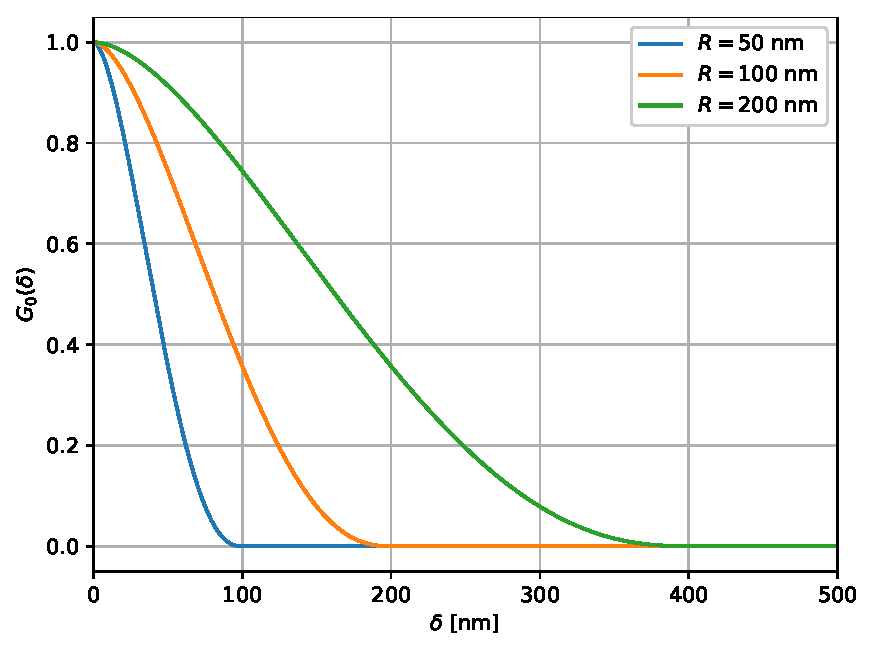
\includegraphics[width=0.5\linewidth]{analytical-G0}
	\caption{Normalized SESANS correlation function $G_0(\delta)$ curves for three dilute mono-disperse solid sphere samples with different radii $R$. The corresponding analytical expression is given by Equation \eqref{eq:sample-G0}.}
	\label{fig:analytical-G0}
\end{figure}

\begin{figure}[h]
	\centering
	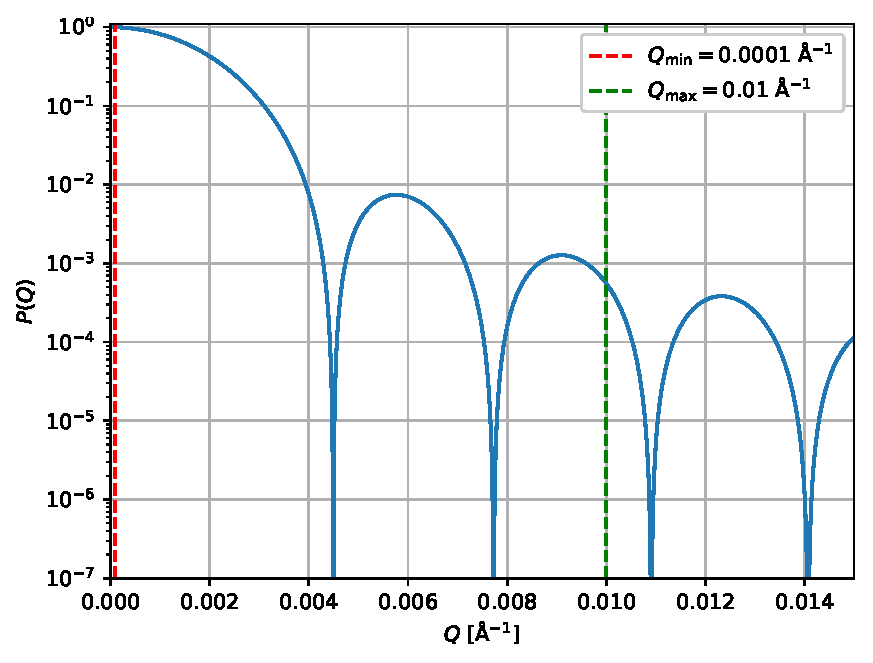
\includegraphics[width=0.5\linewidth]{analytical-P-log}
	\caption{Solid sphere form factor $P(Q)$ for $R = \SI{100}{\nano\meter}$ with $Q_{min}, Q_{max}$ as given by Equation \eqref{eq:sample-form-factor}. It can be seen that for $Q > Q_{max}$, $P(Q) < 10^{-3}$ with its oscillation peaks decreasing in amplitude.}
	\label{fig:analytical-P}
\end{figure}
\subsection{Solid sphere form factor and $Q$-range}
Formulated in terms of wave-vector transfer $Q$ as in regular SANS rather than $\delta$, the relevant $Q$-range of a dilute mono-disperse sample of spheres with radius $R$ can be seen to be largely determined by its form factor $P(Q)$ as $d\sigma(\vec{Q})d\Omega\propto P(Q)$, which is \cite{rekveldt1996}
\begin{equation}
	P(Q) = \left(3\frac{\sin(QR) - QR\cos(QR)}{\left(QR\right)^3}\right)^2\label{eq:sample-form-factor}
\end{equation}
This is a rapidly decaying oscillation with significant values in the range from $Q_{\text{min}} = 0.1/R$ up to $Q_{\text{max}} = 10/R$. This means that in order to determine $G(\delta)$ accurately when measuring a sample that can be described using such a form factor $P(Q)$, a detector should integrate over a proportional $Q$-range.  Figure \ref{fig:analytical-P} shows $P(Q)$ with these limits for $R = \SI{100}{\nano\meter}$.  
